\documentclass[12pt]{beamer}
\usetheme{default}
\usefonttheme{serif}

\usepackage{attrib}

\usepackage[backend=biber, citestyle=authoryear]{biblatex}
\addbibresource{references.bib}

\usepackage{tikz}
\usetikzlibrary{arrows,automata}

\usepackage{minted}

\usepackage{graphicx}

\usepackage{tabularx}
\usepackage{colortbl}

\usepackage{wasysym}

\usepackage{lmodern}

% LTL example
\DeclareMathOperator{\lX}{\textbf{X}}
\DeclareMathOperator{\lU}{\textbf{U}}
\DeclareMathOperator{\lG}{\textbf{G}}
\newcommand{\holds}[2]{\mathrm{holds}_{\left(#1,#2\right)}}

\author{Michael Walker}
\title{Runtime Verification}
\subtitle{A Literature Review}
\date{December, 2014}
\institute{Department of Computer Science\\
  University of York\\
  \texttt{msw504@york.ac.uk}
}

\begin{document}

\begin{frame}[plain]
  \titlepage
\end{frame}

%%%%% 1 Minute (1)

\begin{frame}{Outline}
  \tableofcontents

  \begin{center}
    See the handout for literature references.
  \end{center}
\end{frame}

%%%%% 5 Minutes (6)

\section{Static Analysis is Hard}
\label{sec:statann}

\begin{frame}{Static Analysis}
  \textbf{Static Analysis:} The (fully or partially) automatic process
  of proving properties of programs prior to executing them.

  \visible<2->{
    \begin{itemize}
      \item Type checking
      \item Memory safety
      \item Deadlock/livelock freedom
      \item Schedulability
    \end{itemize}
  }
\end{frame}

\begin{frame}{Rice's Theorem: \small A Nemesis Arises!}
  % PAPERS: rice (corollary b)

  \begin{quote}
    ``If $\mathcal P$ is any property possessed by some, but not all,
    recursively enumerable sets, then there exists no effective
    general method for deciding, given a set $\alpha$ by means of a
    partial recursive function enumerating it, whether or not $\alpha$
    has the property $\mathcal P$.  [\ldots] Of course, there will
    exist special methods for particular functions.''

    \attrib{Rice's Theorem, Corollary B, 1953}
  \end{quote}
\end{frame}

\begin{frame}{Practical Static Analysis: \small Defeating Rice}
  Rice's theorem:
  \begin{itemize}
    \item applies to Turing machines,
    \item refers to exact results,
    \item refers to a fully automatic analysis.
  \end{itemize}

  \visible<2->{
    \vspace{0.25cm}

    We can:
    \begin{itemize}
      \item use more specific systems,
      \item use approximations,
      \item introduce human contribution.
    \end{itemize}
  }
\end{frame}

%%%%% 15 Minutes (21)

\section{Runtime Verification}
\label{sec:runver}

\begin{frame}
  \begin{center}
    \Large Static analysis is getting harder

    \visible<2>{
      \vspace{0.25cm}
      \ldots but maybe there is another way.
    }
  \end{center}
\end{frame}

\begin{frame}{Runtime Verification}
  % NON-PAPERS: rv01

  \begin{quote}
    ``\ldots is to investigate whether the use of lightweight formal
    methods applied during the execution of programs is a viable
    complement to the current heavyweight methods proving programs
    correct always before their execution, such as model checking and
    theorem proving.''

    \attrib{K. Havelund \& G. Rosu, RV'01}
  \end{quote}

  There are two main foci of work: design by contract and trace
  analysis.
\end{frame}

%%%%%%%%%% 7 Minutes (13)

\subsection{Design by Contract}
\label{sec:runver-dbc}

\begin{frame}
  \begin{center}
    \Large Design by Contract
  \end{center}
\end{frame}

\begin{frame}{Design by Contract}
  % PAPERS: eiffel

  \begin{itemize}
    \item Introduced in 1988 in Eiffel \parencite{eiffel}.
    \item Functions have associated pre- and postconditions.
    \item Preconditions are assumed true when the function is called.
    \item Postconditions must be true if the function terminates
      and the precondition was met.
  \end{itemize}

  \visible<2->{
    \vspace{0.25cm}

    Contracts can be:

    \begin{itemize}
      \item simply assumed; or
      \item verified statically; or
      \item verified at runtime, by instrumenting function calls.
    \end{itemize}
  }
\end{frame}

\begin{frame}{Contract Languages}
  \begingroup
  \renewcommand{\arraystretch}{2}
  \begin{tabularx}{\textwidth}{|X|c|c|}
    \hline
    & Learning curve & Automated reasoning\\

    \hline
    \textbf{DSL\footnotemark} & \cellcolor{red!25} {\Large \frownie} &
    \cellcolor{green!25} {\Large \smiley}\\

    \hline
    \textbf{Host} & \cellcolor{green!25} {\Large \smiley} &
    \cellcolor{red!25} {\Large \frownie}\\

    \hline
  \end{tabularx}
  \endgroup

  \footnotetext[1]{Domain Specific Language}
\end{frame}

\subsubsection{Domain-specific Languages}
\label{sec:runver-dbc-dsl}

\begin{frame}[fragile]{Contract Languages: \small JML \parencite{jml}}
  % PAPERS: jml

  JML\footnotemark{} has

  \begin{itemize}
    \item data and loop invariants,
    \item ghost variables,
    \item method frame specification,
    \item model methods.
  \end{itemize}

  Contracts can be compiled to executable code, producing runtime
  monitors.

  \footnotetext[2]{Java Modelling Language}
\end{frame}

\begin{frame}{JML Example}
  % Horrible, but it works.
  \inputminted[fontsize=\footnotesize, lastline=10]{java}{jmlstack.java}
  \vspace{-1cm}
  \textbf{\inputminted[fontsize=\footnotesize, firstline=11, lastline=14]{java}{jmlstack.java}}
  \vspace{-0.33cm}
  \inputminted[fontsize=\footnotesize, firstline=15]{java}{jmlstack.java}
\end{frame}

\begin{frame}{Contract Languages: \small BCSL / BML \parencite{bcsl}}
  % PAPERS: bcsl, bml

  BCSL\footnotemark{} (later BML\footnotemark; \cite{bml})

  \begin{itemize}
    \item JML analogue for Java bytecode
    \item Can be produced from JML
    \item Developed for the possibility of proof-carrying code
    \item Compact binary representation of contracts
  \end{itemize}

  \footnotetext[2]{Bytecode Specification Language}
  \footnotetext[4]{Bytecode Modelling Language}
\end{frame}

\begin{frame}[fragile]{BML Example}
  \begin{verbatim}
{| requires #2 > 0
   ensures #2 == \old(#2) - 1
   ensures \result == \old(#3) |}
  \end{verbatim}

  \textbf{\large Compact encoding}\smallskip

  Predicates: \textbf{30 bytes} (compared with \textbf{80}).

  \vspace{0.25cm}

  Predicates + metadata: \textbf{50 bytes}.
\end{frame}

\begin{frame}[fragile]{BML Example}
  \footnotesize
  \begin{center}
  \begin{tikzpicture}[level/.style={sibling distance=5cm/#1, level distance=1.33cm}]
    \node (a) {\&\&}
      child {node (b) {==}
        child {node (c) {\#}
          child {node (d) {2}}
        }
        child {node (e) {-}
          child {node (f) {old}
            child {node (g) {\#}
              child {node (h) {2}}
            }
          }
          child {node (i) {int}
            child {node (j) {1}}
          }
        }
      }
      child {node (k) {==}
        child {node (l) {result}}
        child {node (m) {old}
          child {node (n) {\#}
            child {node (o) {3}}
          }
        }
      };

    \path (a) -- (b);
    \path (a) -- (k);
    \path (b) -- (c);
    \path (b) -- (e);
    \path (c) -- (d);
    \path (e) -- (f);
    \path (e) -- (i);
    \path (f) -- (g);
    \path (g) -- (h);
    \path (i) -- (j);
    \path (k) -- (l);
    \path (k) -- (m);
    \path (m) -- (n);
    \path (n) -- (o);
  \end{tikzpicture}
  \end{center}
\end{frame}

\begin{frame}[fragile]{BML Example}
  \footnotesize
  \begin{center}
  \begin{tikzpicture}[level/.style={sibling distance=6cm/#1, level distance=1.33cm}]
    \node (a) {0x02}
      child {node (b) {0x08}
        child {node (c) {0x80}
          child {node (d) {0x0002}}
        }
        child {node (e) {0x28}
          child {node (f) {0x99}
            child {node (g) {0x80}
              child {node (h) {0x0002}}
            }
          }
          child {node (i) {0x40}
            child {node (j) {0x00000001}}
          }
        }
      }
      child {node (k) {0x08}
        child {node (l) {0x52}}
        child {node (m) {0x99}
          child {node (n) {0x80}
            child {node (o) {0x0003}}
          }
        }
      };

    \path (a) -- (b);
    \path (a) -- (k);
    \path (b) -- (c);
    \path (b) -- (e);
    \path (c) -- (d);
    \path (e) -- (f);
    \path (e) -- (i);
    \path (f) -- (g);
    \path (g) -- (h);
    \path (i) -- (j);
    \path (k) -- (l);
    \path (k) -- (m);
    \path (m) -- (n);
    \path (n) -- (o);
  \end{tikzpicture}

  \textbf{0x020880000228998000024000000001085299800003}
  \end{center}
\end{frame}

\subsubsection{Re-using the Host Language}
\label{sec:runver-sbc-aop}

\begin{frame}{Host Language}
  \begin{itemize}
    \item Rather than define a new contract language, re-use the host
      language.

    \item May define high-level functions approximating a DSL.

    \item Easy to use for runtime monitors.

    \item Difficult to use for static analysis.
  \end{itemize}
\end{frame}

\begin{frame}{Host Language: \small jContractor \parencite{jcontractor}}
  % PAPERS: jcontractor

  jContractor specifies contracts for methods in separate methods
  following a naming scheme, with checking implemented by on-the-fly
  bytecode manipulation.

  \begin{itemize}
    \item Overhead is only incurred if the code is run with
      jContractor.

    \item Conversely, only checks contracts when explicitly told to.

    \item This may make it more suitable for developmental purposes
      than debugging ``in the wild''.
  \end{itemize}
\end{frame}

%%%%%%%%%% 7 Minutes (20)

\subsection{Trace Analysis}
\label{sec:runver-trace}

\begin{frame}
  \begin{center}
    \Large Trace Analysis
  \end{center}
\end{frame}

\begin{frame}{Trace Analysis}
  % Overview of traces, quote seminal paper (Hoare?), explain how we
  % can generate traces by triggering events at program points
  % (find good paper), and how we can specify properties of programs
  % as properties of traces.

  % PAPERS: cspthy

  \begin{itemize}
    \item Introduced in 1984 in CSP\footnotemark{} \parencite{cspthy}.
    \item Execution of a program specified in terms of a sequence of events.
  \end{itemize}

  \visible<2->{
    \vspace{0.25cm}

    Traces can be used to:

    \begin{itemize}
      \item reason about relations between programs; or
      \item monitor adherence to a
        specification \parencite{efficient}.
    \end{itemize}
  }

  \footnotetext[5]{Communicating Sequential Processes}
\end{frame}

\begin{frame}{Motivating Example: \small See (\cite{compensate} \S7)}
  \begin{itemize}
    \item Financial transaction systems need fraud detection and
      handling.
    \item Users can be considered separate `processes' with their own
      traces.
    \item Monitoring happens on a per-user basis, and fraud is
      characterised by unusual behaviour (sub-traces).
  \end{itemize}

  It's not easy to see how to specify this with contracts.
\end{frame}

\begin{frame}{Trace Logics: \small EREs \parencite{eres}}
  EREs\footnotemark{} are one way of expressing properties of traces,
  where trace elements consist of one of a few well-defined values.

  \vspace{0.25cm}

  EREs add complementation to regular expressions.

  \vspace{0.25cm}

  \textit{e.g.} an iterator must always have items remaining before
  reading, so valid traces are of the form,

  \begin{center}
    \texttt{(hasNext next)*}
  \end{center}

  \footnotetext[6]{Extended Regular Expressions}
\end{frame}

\begin{frame}{Trace Logics: \small LTL \parencite{ltl}}
  LTL\footnotemark{} is a modal logic,

  \begin{align*}
    \lX p &\equiv \mbox{$p$ is true in the next time step}\\
    w \models \lX p &\Leftrightarrow w_{1} \models p\\\\
    p \lU q &\equiv \mbox{$p$ is true until $q$ becomes true}\\
    w \models p \lU q &\Leftrightarrow \left(\exists i \geq 0,\ w_{i}
      \models p \land \forall 0 \leq k < i,\ w_{k}
      \models q\right)\\
  \end{align*}

  \textit{e.g.} checking that a process doesn't undergo lock
  reversal \parencite{hask},

  \begin{align*}
    \lG \lnot\left(\holds{j}{x} \land \lnot \holds{j}{y} \land
      \left(\holds{j}{x} \lU \holds{j}{y}\right)\right)\\
  \end{align*}

  \footnotetext[7]{Linear Temporal Logic}
\end{frame}

%%%%%%%%%% 1 Minutes (21)

\subsection{Contracts + Traces?}
\label{sec:runver-tbc}

\begin{frame}
  \begin{center}
    \Large Contracts and traces let us specify properties in different
    ways, but we can combine them.
  \end{center}
\end{frame}

\begin{frame}{Trace Monitors}
  We can define a trace monitor as a state machine.

  \begin{center}
    \begin{tikzpicture}[->, auto, node distance=8cm]
      \node[initial,state] (A)              {$s_{A}$};
      \node[state]         (B) [right of=A] {$s_{B}$};

      \path (A) edge [loop above] node {foo()} (A)
                edge [bend left]  node {bar()} (B)
            (B) edge [bend left]  node {baz()} (A);
    \end{tikzpicture}
  \end{center}
\end{frame}

\begin{frame}{Augmented Trace Monitors}
  State transitions can include pre- and
  postconditions \parencite{unified}.

  \begin{center}
    \begin{tikzpicture}[->, auto, node distance=8cm]
      \node[initial,state] (A)              {$s_{A}$};
      \node[state]         (B) [right of=A] {$s_{B}$};

      \path (A) edge [loop above] node {pre / foo() / post} (A)
                edge [bend left]  node {pre / bar() / post} (B)
            (B) edge [bend left]  node {pre / baz() / post} (A);
    \end{tikzpicture}
  \end{center}
\end{frame}

%%%%% 4 Minutes (25)

\section{Conclusions}
\label{sec:conc}

\begin{frame}
  \begin{center}
    \only<1>{
      \Large Static analysis and runtime verification give different
      viewpoints.
    }

    \only<2>{
      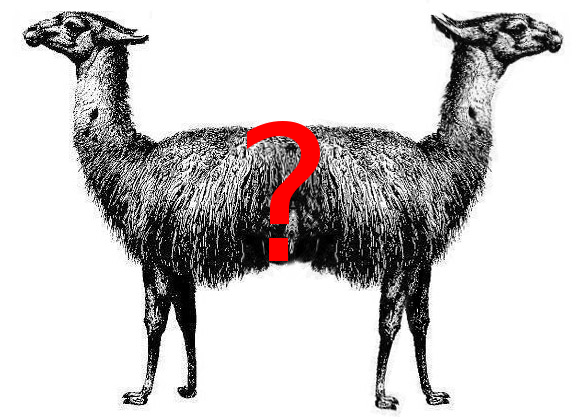
\includegraphics[width=0.75\textwidth]{pushmi-pullyu.png}
    }
  \end{center}
\end{frame}

\begin{frame}{Combined approaches}
  % PAPERS: statver, unified

  Work has been done on:

  \begin{itemize}
    \item Static verification of dynamically-detected
      invariants \parencite{statver},

    \item Using static verification to simplify or even eliminate
      monitoring obligations \parencite{unified}.
  \end{itemize}
\end{frame}

\begin{frame}
  \begin{center}
    \Large Successes \& open problems
  \end{center}
\end{frame}

\begin{frame}{Successes}
  % PAPERS: valgrind, compensate, datarace, addrsan

  \begin{itemize}
    \item Valgrind \parencite{valgrind}
    \item Memory error detection \parencite{addrsan}.
    \item Data race detection \parencite{datarace}.
    \item Low-overhead monitoring \parencite{compensate}.
  \end{itemize}
\end{frame}

\begin{frame}{Open Problems}
  \begin{itemize}
    \item Simultaneous compensation \parencite{compensate}.
    \item Static/runtime boundary assumptions \parencite{explicit}.
  \end{itemize}
\end{frame}

\begin{frame}{Runtime Verification: \small A Summary}
  \begin{itemize}
    \item<1-> Only reasons about the current execution
    \item<1-> ``More decidable'' than static analysis
    \item<2-> But not incompatible with static analysis!
    \item<3-> Still a lot to be done in efficient and safe monitoring
      / error recovery
  \end{itemize}
\end{frame}

\begin{frame}{Questions?}
  \vspace{4.5cm}

  \footnotesize
  \textbf{Q:} What is the two-headed creature a few slides back?\\
  \textbf{A:} A pushmi-pullyu, from \textit{The Story of Doctor Dolittle}.

  \begin{quote}
    ``I notice,'' said the duck, ``that you only talk with one of your
    mouths. Can't the other head talk as well?''

    ``Oh, yes,'' said the pushmi-pullyu. ``But I keep the other mouth
    for eating---mostly. In that way I can talk while I am eating
    without being rude. Our people have always been very polite.''
  \end{quote}
\end{frame}

\end{document}